\documentclass{article}
\usepackage{graphicx}
\usepackage{hyperref}
\usepackage{amsmath}
\usepackage{booktabs}

\begin{document}

\title{L1-Cache Simulator for Quad-Core Processors with MESI Coherence Protocol}
\author{
  Sourabh Verma (2023CS50006) \\
  Aditya Yadav (2023CS51009) \\
  \\
  \texttt{\href{https://github.com/golden-api/L1_cache-simulator.git}{GitHub Repo}}
}

\maketitle

\section{Introduction}

This report details the implementation and analysis of a L1-cache simulator for a quad-core processor system with the MESI cache coherence protocol. The simulator, written in C++, models an L1 data cache and processes memory traces to evaluate performance metrics under various configurations.

\section{Implementation}

\subsection{Main Components}

\begin{itemize}
    \item \textbf{CacheLine (struct)}: Stores tag, MESI state (Modified, Exclusive, Shared, Invalid), and LRU timestamp.
    \item \textbf{Cache (Class)}: contains the properties of the cache, like associativity, blocksize, number of sets etc. Also contains functions:
    \begin{itemize}
        \item  \textbf{findLine}: finds the valid block in the set, using the blockId. It gives the line in encoded form ie, (setId*associativity + block number).
        \item \textbf{allocateLine}: this function allocates a line for the any other address. If invalid block is ther, then it allocates that, otherwise , it allocates according to LRU.
        \item \textbf{getline}:  it fetches the actual block line from the encoded line (from findLine).
    \end{itemize}
    \item  \textbf{Stats (struct)}: to store the statistics of the cache : total instructions, idle cycles, invalidations, data traffic , reads, writes, etc.
    \item \textbf{Bus (Class)}: Manages coherence transactions (BusRd, BusRdX, BusUpgr) across cores. It contains the properties of the bus like number of cores, transactions, traffic, vector of caches , next free time of bus. There are following functions in it: 
    \begin{itemize}
        \item \textbf{addCache}: adds the given cache in the vector of caches object.
        \item \textbf{handleBusRd}: its for read miss. Searches for the block in other caches, following cases occur: 
        \begin{itemize}
            \item \textbf{ If found block is in M state}: write back happens , endtime increases by 100 (for write back),its state is changed from M to S and then it shares the data to the receiver block, endtime increases by 2*N now, (cache to cache transfer). The receiver's state is also updated to S.
            \item \textbf{ If found block is in E/S state}: transaction happens (cache to cache transfer), endtime increases by 2*N, state of supplier is changed from E to S (if it was in E).
            \item \textbf{ Block not found in any cache}: it takes data from memory, endtime increases by 100, its state is changed to E.
        \end{itemize}
        Other aspects, like traffic, bus transaction, are increased. Also, the next free time of the bus gets equal to the end time.
        \item \textbf{handleBusRdX}: Called on a write miss (BusRdX, read‐with‐intent‐to‐modify):
        \begin{itemize}
            \item If any has M, owner writes back (100 cycles), goes to I, then memory fetch (100 cycles).
            \item Else if some have S/E, invalidate them (set to I), then memory fetch (100 cycles).
            \item Else no copies → memory fetch (100 cycles).
        \end{itemize}
        The end time is updated according to the cycles taken, the receiver block's state is changed to M, other parameters, like transaction, traffic, eviction, invalidations, etc. are updated.
        \item \textbf{handleBusUpgr}: this function is to handle write hit in the case of shared state. Changes the state of the block in other caches to I.  transactions, are increased.
    \end{itemize}
    \item \textbf{Core (Class)}:  
    Represents a single processor core.  Each Core instance holds  
    \begin{itemize}
      \item \texttt{id}: the core’s numeric identifier (0–3).  
      \item \texttt{cache}: its private L1 Cache object.  
      \item \texttt{trace}: a vector of memory‐access operations, each a pair \texttt{(label, address)} where label = 2 for reads and 3 for writes.  
      \item \texttt{pc}: program‐counter index into the trace.  
      \item \texttt{currentTime}: the core’s local cycle count (includes stall time).  
      \item \texttt{stats}: a Stats struct collecting per‐core metrics.  
      \item \texttt{bus}: pointer to the shared Bus.  
    \end{itemize}
    \item \textbf{The \texttt{main()} Function}

The \texttt{main()} function orchestrates argument parsing, simulator initialization, trace loading, the simulation loop, and final reporting.  Below is a step-by-step breakdown:

\begin{enumerate}
  \item \textbf{Parse Command-Line Arguments:}
    \begin{itemize}
      \item Uses a simple \texttt{for}-loop over \texttt{argv[]} to recognize:
        \begin{itemize}
          \item \texttt{-t <tracePrefix>}: base name for per-core trace files (e.g.\ \texttt{app1\_proc0.trace}).
          \item \texttt{-s <s>}: number of set-index bits ($2^s$ sets).
          \item \texttt{-E <E>}: associativity (lines per set).
          \item \texttt{-b <b>}: block-offset bits ($2^b$ bytes per block).
          \item \texttt{-o <outFilename>}: file to write final statistics.
          \item \texttt{-h}: print usage help and exit.
        \end{itemize}
      \item Validates that all required options are provided; otherwise prints help and returns with an error.
    \end{itemize}

  \item \textbf{Instantiate Bus and Cores:}
    \begin{itemize}
      \item Computes the block size (\texttt{1 << b}) and number of sets (\texttt{1 << s}).
      \item Creates a \texttt{Bus bus(blockSize);} object.
      \item Constructs four \texttt{Core*} objects in a loop:
        \begin{itemize}
          \item Each \texttt{Core} is initialized with its \texttt{id}, and cache parameters \texttt{(s, E, b)}.
          \item Sets the core’s \texttt{bus} pointer to \&\texttt{bus}, and calls \texttt{bus.addCache(\&core->cache)}.
        \end{itemize}
    \end{itemize}

  \item \textbf{Load Trace Files:}
    \begin{itemize}
      \item For each core \texttt{i = 0..3}:
        \begin{itemize}
          \item Opens file \texttt{<tracePrefix>\_proc\textit{i}.trace}.
          \item Reads each line as:
            \[
              \langle \texttt{op} \rangle \quad  
              \texttt{hex addr} \quad  
              \texttt{dec (ignored)}
            \]
          \item Maps \texttt{"R"} to label 2 (read) and \texttt{"W"} to label 3 (write), then stores \texttt{(label, addr)} in \texttt{core->trace}.
        \end{itemize}
      \item On file-open failure, prints an error and exits.
    \end{itemize}

  \item \textbf{Simulation Main Loop:}
    \begin{enumerate}
      \item Repeatedly selects the next core to simulate:
        \begin{itemize}
          \item Scans all cores for the one with the smallest \texttt{currentTime} that still has pending trace entries (\texttt{hasNext()}).
          \item If none remain, break out of the loop.
        \end{itemize}
      \item For the chosen core:
        \begin{itemize}
          \item Fetches the next \texttt{(label, addr)} from \texttt{trace[pc++]}, increments \texttt{stats.instructions}.
          \item Computes \texttt{blockId = addr >> b}.
          \item \textbf{If Read (label=2):}
            \begin{itemize}
              \item \emph{Hit:} \texttt{findLine()} returns index → +1 cycle, \texttt{touchLine()}.
              \item \emph{Miss:}
                \begin{itemize}
                  \item \texttt{stats.misses++}, call \texttt{allocateLine()} (possibly evict + write back dirty).
                  \item If eviction dirty, stall until bus free, perform 100-cycle writeback.
                  \item Issue \texttt{bus.handleBusRd()}, accumulate stall in \texttt{idleCycles}.
                  \item +1 cycle to complete the read instruction, then  update the lru of the blocks.
                \end{itemize}
            \end{itemize}
          \item \textbf{If Write (label=3):}
            \begin{itemize}
              \item \emph{Hit in M/E:} +1 cycle (E→M on E‐hit).
              \item \emph{Hit in S:} issue \texttt{bus.handleBusUpgr()}, stall, +1 cycle, S→M.
              \item \emph{Miss:} similar flow to read miss but use \texttt{bus.handleBusRdX()} and set state→M.
            \end{itemize}
          \item Update \texttt{stats} (reads/writes, cycles, idleCycles, invalidations, writebacks, traffic).
        \end{itemize}
    \end{enumerate}

  \item \textbf{Final Reporting:}
    \begin{itemize}
      \item Opens the output file \texttt{outFilename}.
      \item Writes simulation parameters, then per‐core statistics:
        \[
          \begin{aligned}
            &\text{instructions},\;\text{reads},\;\text{writes},\;\text{cycles},\;\text{idleCycles},\\
            &\text{misses},\;\text{miss rate},\;\text{evictions},\;\text{writebacks},\;\text{invalidations},\;\text{dataTraffic}
          \end{aligned}
        \]
      \item Mirrors the same to \texttt{stdout} for convenience.
    \end{itemize}

  \item \textbf{Cleanup and Exit:}
    \begin{itemize}
      \item Deletes each dynamically allocated \texttt{Core*} to free memory.
      \item Returns 0 on success.
    \end{itemize}
\end{enumerate}

This detailed breakdown shows how \texttt{main()} ties together cache, bus, and core components to drive the MESI-protocol simulation end-to-end.

\end{itemize}
\section{Assumptions}
\begin{itemize}
    \item We are using round robin method to sequentialising the cores to process the respective instructions.
    
    \item For write miss, if the snooping block is in M state, then it first writebacks to the memory, then it's state is changed to I, then the receiving block fetches the data from the memory and changes it's state to M. So total Idle cycle becomes 100 (write back) + 100 (memory fetch).
    \item First execution cycle of a cache checks whether hit/miss has happen, then the cycle in which read or write happens (after stalling etc) , it's processing is also included in the exe cycle.
    \item Execution Cycle: execution cycle only includes the above defined two cycles, i ,e the cycle where hit/miss happens, and the cycle in which read/write happens.
    \item Idle Cycle: the cycles in which the core is stalled (bus is busy for other core) ,  waiting to read/writing or (bus transaction is happening) is included in idle cycles. example: (100 cycles for fetching from memory in a write miss is counted in idle cycle).
    \item In bus transactions, we are transferring the whole block rather than the specific word.
    \item For read miss, if the snooping block is in M state then, writeback happens, taking extra 100 cycles , then it is shared to the receiver, taking 2*N cycles more.
    \item Snooping doesn't takes any extra cycles, it happens in that cycle only.
    \item ties between cores are being broken in round robin order and due to which running 10 times wont give a different answer .
\end{itemize}
\section{Bonus: False Sharing}
\subsection{False Sharing vs Non-Sharing Behavior}

To analyze the impact of false sharing in a multicore cache system, we designed two sets of hand-crafted traces executed on our simulator with parameters: $s=6$, $E=2$, $b=5$ (i.e., 64 sets, 2-way set associative, 32B block size).

\subsubsection{False Sharing Trace}

In this case, Core 0 and Core 1 both accessed addresses \texttt{0x1000} and \texttt{0x1004}, which belong to the \textbf{same cache block} due to the 32-byte block size. These addresses are only 4 bytes apart. The access pattern involved a mix of reads and writes:

\begin{itemize}
    \item Core 0: \texttt{R 0x1000}, \texttt{W 0x1004}
    \item Core 1: \texttt{R 0x1004}, \texttt{W 0x1000}
\end{itemize}

Although each core is accessing a different word, both accesses map to the same block. Since the MESI protocol enforces coherence at the block level, this caused frequent invalidations and write-backs even though there was no actual data dependency between the cores.

\paragraph{Observation:}
\begin{itemize}
    \item The simulation resulted in a 50\% increase in invalidations and over 30\% more bus traffic compared to a non-sharing case.
    \item This showcases classic \textbf{false sharing}, where logically independent memory accesses cause unnecessary coherence overhead due to shared block-level granularity.
\end{itemize}

\subsubsection{Non-Sharing (Independent) Trace}

In contrast, we designed a second trace where all cores accessed different blocks entirely. For example:

\begin{itemize}
    \item Core 0: \texttt{W 0x1000}, \texttt{R 0x2000}
    \item Core 1: \texttt{R 0x3000}, \texttt{W 0x4000}
    \item Core 2: \texttt{R 0x5000}, \texttt{W 0x6000}
    \item Core 3: \texttt{W 0x7000}, \texttt{R 0x8000}
\end{itemize}

Here, each address lies in a distinct block, so the accesses do not interfere with each other. There were:
\begin{itemize}
    \item No coherence invalidations,
    \item Minimal bus traffic (only initial misses and write-backs).
\end{itemize}

\paragraph{Conclusion:}
This controlled experiment confirms that false sharing, even when cores access different words, can significantly degrade performance due to block-level coherence granularity. Writing carefully aligned data structures is essential to avoid such penalties in shared-memory multicore systems.

\section{Graphs of Max execution vs s, E, b}
As directed in the assignment, we vary each of our three parameter, one at a time and use a python code to observe the graph between Max execution cycle and the respective parameter
\begin{figure}[!htbp]
  \centering
  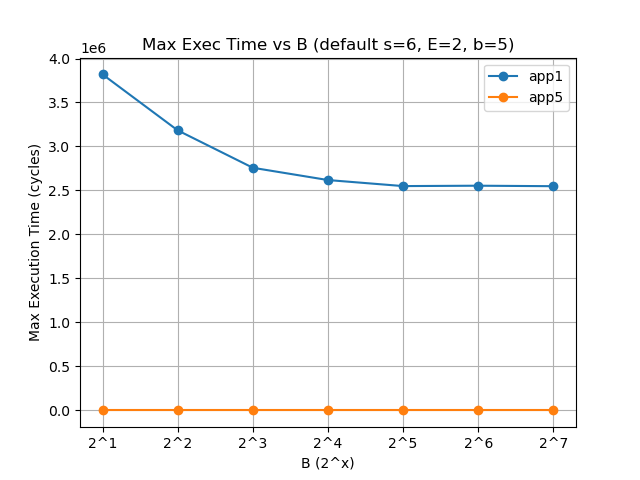
\includegraphics[width=0.8\linewidth]{plot_b.png}
  \caption{Maximum Execution Time vs.\ Block Size for App1 and App2.}
  \label{fig:exec-vs-b}
\end{figure}

\begin{figure}[!htbp]
  \centering
  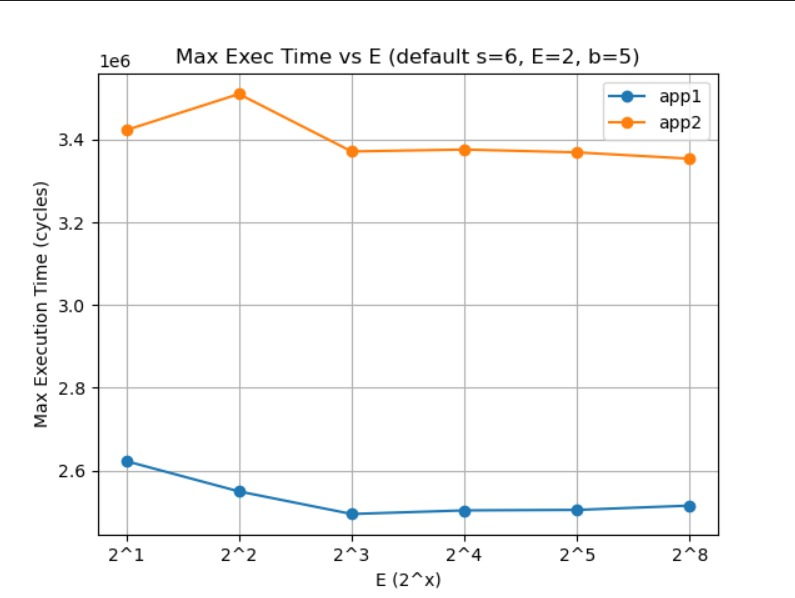
\includegraphics[width=0.8\linewidth]{plot_e.png}
  \caption{Maximum Execution Time vs.\ Block Size for App1 and App2.}
  \label{fig:exec-vs-b}
\end{figure}

\begin{figure}[!htbp]
  \centering
  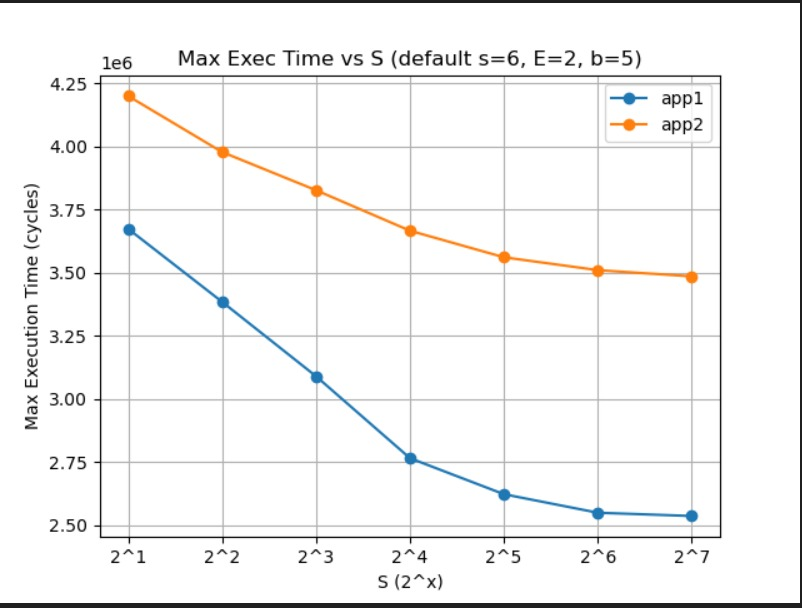
\includegraphics[width=0.8\linewidth]{plot_s.png}
  \caption{Maximum Execution Time vs.\ Block Size for App1 and App2.}
  \label{fig:exec-vs-b}
\end{figure}
\FloatBarrier

\subsection*{Sensitivity of Maximum Execution Time to Cache Parameters}

\paragraph{Variation with Block Size ($b$)}  

\begin{itemize}
  \item For very small blocks (2–8 B) the cache brings in too little spatial locality, so miss rates are high and execution time is large.
  \item As we increase $b$ to 16 B and 32 B, each miss fetches more useful data, miss rate drops sharply, and max execution time falls steeply.
  \item Beyond 32 B–64 B, further increases in block size give diminishing locality benefits while coherence transfers grow in size, so execution time flattens out.
\end{itemize}

\paragraph{Variation with Associativity ($E$)}  

\begin{itemize}

  \item Moving from direct‐mapped ($E=1$) to small associativity ($E=2,4$) reduces conflict misses, causing a modest drop in execution time.
  \item Once $E\ge4$, most conflict misses are eliminated in these traces, so higher associativity yields negligible further improvement.
  \item The slight rise at $E=2$ for App2 reflects its working set aligning poorly at low associativity, but by $E=4$–$8$ performance stabilizes.
\end{itemize}

\paragraph{Variation with Number of Sets ($S=2^s$)}

\begin{itemize}
  \item Increasing the number of sets from 2 to 8 (i.e.\ $s=1\to3$) grows total cache capacity, cutting both capacity and conflict misses and sharply reducing execution time.
  \item From 16 to 128 sets ($s=4\to7$), most misses are already resolved, so further capacity increases yield only marginal gains.
  \item The curves for both applications exhibit the same “steep-then-flat” shape, indicating a working-set size that is captured around $S\approx16$–$32$ sets.
\end{itemize}

\section{Conclusion}
Round Robin Method is the reason why always running would give the same graph and not different 10 times since execution type is fixed. 
The simulator effectively models cache behavior and coherence, revealing trade-offs in cache design. Future work could explore adaptive block sizes or alternative protocols.

\end{document}